\documentclass[../main.tex]{subfiles}


\begin{document}
\raggedright
The interface will consist of three different types of users; The Students, the Secretary and the Scrutiny Committee. There will be other third party users who will get the data from the student records such as the professors and personal tutors. 

\subsection{Student Panel}
The student panel will consist of three main components; They should be able to submit a new circumstance form, access any previously submitted form and lastly check the status(described under Scrutiny Committee Panel) for any new feedbacks or requests from the scrutiny committee and upload a response or evidence as required. As stated in the previous section, the students should be able to login with their university accounts making it easy to access from within the portal. However, this may turn out to be difficult as accessing the university Intranet would be a security risk to the University.

\subsection{Secretary Panel}
This panel will be a little more detailed than the student panel. The panel would notify the secretary by email when a new form is received. The secretary can then process the form and take it to the next scrutiny panel meeting. The panel would also allow searching and filtering of all the forms submitted by all students. The scrutiny committee will have access to the system as well which allows all users in the meeting to view the form and decide its fate. Once the scrutiny committee has decided, the secretary will be able to change the status of the project to either \textit{Rejected} or \textit{Approved}. Alternately, if the scrutiny committee decides they would like more proof, the secretary would be able to request these from the student directly from the panel. As exporting data was one of the requirements, the interface should provide the secretary and the scrutiny panels a button through which they can print and save the form as a PDF document. 

\subsection{Scrutiny Panel}
This would be a read-only portal where the members of the scrutiny committee can access and read all the data and submit their concerns to the secretary under their minutes for the meeting. This follows the same procedure they already have in place where the secretary would be the one in contact with the student. Figure \ref{fig:mockup} shows an example of the scrutiny panel's read only access

	\begin{figure}[H]
        \center{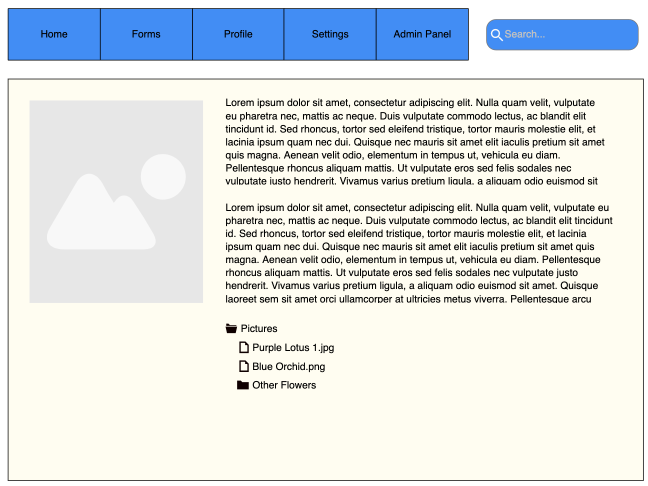
\includegraphics[scale=1.2]
        {images/moqup.png}}
        \caption{\label{fig:mockup} Portal mock-up}
      \end{figure}

\end{document}
